\documentclass[12pt]{article}

%—————————— Packages ———————————————————————————
\usepackage[T1]{fontenc}
\usepackage{amsmath, amssymb}
\usepackage{graphicx}
\usepackage{dsfont}
\usepackage{authblk}
\usepackage{geometry}
\usepackage{enumitem}
\usepackage{booktabs}
\usepackage{hyperref}
\usepackage{array}
\usepackage{multirow}
\usepackage{listings}
\usepackage{siunitx}      % For \SI{...}{...}
\sisetup{
  per-mode = symbol, % utilise un slash au lieu de l’exposant -1
  per-symbol = /     % explicite : le symbole est "/"
}
\DeclareSIUnit{\MWh}{\mega\watt\hour}
\usepackage{microtype}    % Optional but recommended
\usepackage{float}
\usepackage{booktabs,tabularx,ragged2e}
\usepackage{mathtools}        % \mathclap, \makebox
\usepackage{cleveref} 
\usepackage[square,authoryear]{natbib}
\usepackage{caption}  
\usepackage{textcomp}
\usepackage{tikz}
\usetikzlibrary{shapes,arrows,positioning,fit,backgrounds,calc}   
\DeclareSIUnit{\EUR}{\text{\texteuro}}
\DeclareSIUnit{\MEUR}{\mega\EUR}



\captionsetup{justification=centering} % pour \cref, \Cref
\newcommand{\EURM}[1]{\SI{#1}{\mega\euro}} % "million d'euros" rapide
\newcommand{\lbl}[2]{%
  \underbrace{\mathstrut #1}_{\mathclap{\text{#2}}}}

\newlength{\BracketW}         % largeur interne du grand crochet
\setlength{\BracketW}{.86\linewidth}   % ajustez 0.80–0.90 si besoin
\newcolumntype{L}{>{\raggedright\arraybackslash}p{3.6cm}} % fixed-width, left-aligned
\newcolumntype{Y}{>{\RaggedRight\arraybackslash}X}        % auto-sizing, left-aligned





%—————————— Title ——————————————————————————————
\title{Flexibility as a Driver of Regionalized Power Systems:
A Multi-Regional Optimization Framework\\}

\author[1]{Théotime Coudray}
\author[2]{Sandrine Michel}
\affil[1]{Université de Versailles Saint-Quentin-en-Yvelines, UMI SOURCE}
\affil[2]{Université de Montpellier, UMR 5281 ART-Dev}
\date{ }

\bibliographystyle{elsarticle-harv}
\begin{document}
\maketitle

\begin{abstract}
In the context of the ongoing Energy Transition (ET), power system flexibility has emerged as a critical requirement for integrating increasing shares of Variable Renewable Energies (VREs) into electricity mixes. Because these resources are inherently location-specific, their large-scale deployment calls for a rethinking of how the balance between supply and demand is achieved. In this paper, we propose a multi-regional optimization framework to balance residual load using existing flexibility tools, including dispatchable generation, storage, demand response (DR), and inter-regional exchanges. Applying this framework to a cluster of four southern French regions for the full year 2023, we find that the residual load is met by an overwhelmingly low-carbon dispatchable mix dominated by nuclear baseload, that inter-regional exchanges constitute the primary flexibility channel and generate substantial economic value through congestion rents (\(\sim 0.91\) billion euros). We confirm the robustness of these findings through a dedicated sensitivity analysis spanning the hydro energy budget, the DR rebound parameter, and inter-annual variability (2022 versus 2023). These results suggest that introducing an intermediate regional layer for the operation and coordination of power system flexibility could be beneficial from both a technical and an economic perspective.
\end{abstract}



\begin{center}
\textbf{Keywords:} Power System; Multi-Scale; Variable and Renewable Energies (VRE); Residual Load; Flexibility; Energy Modeling
\end{center}

\vspace{1em}


%—————————— Sections ————————————————————————————
\section{Introduction}

\subsection{Context}

\paragraph{}
Energy transition (ET) generally refers to a change in the structure of energy resources used in the production mix. However, the concept can  have at least two other broader meanings. It may refer to the period during which the adoption of new energy resources reaches a significant share of the mix and triggers a reorganization of the energy system required to exploit them \citet{smil2010}. More generally, it may denote the time during which this new way of producing energy reshapes the entire economy \citep{crafts2004,bergquist2023}. These durations have been estimated to range from about thirty years to several decades, and in some cases up to a century or more \citep{fouquet2016}. Past ETs therefore teach us that the organization of energy systems, while adapting, persists long before they fully transform.

\paragraph{}
According to \citet{smil2010}, the current transition is characterized by the objective of decarbonizing energy. Achieving this objective opens a new long-term phase of co-adaptation between emerging technologies and the economic organization of the energy system \citep{grubler2012}. Nowadays, electricity plays an increasingly central role in energy systems: both its demand and supply grow faster than any other energy use \citep{iea2025}. Variable Renewable Energies (VREs) effectively renew the terms for achieving instantaneous balance between supply and demand, requiring the reorganization of electrical systems. Flexibility is one such requirement.

\subsection{Flexibility}

\paragraph{}
In the pre-VRE technological regime, balancing capabilities were embedded in controllable supply portfolios, operational hierarchies, and nationally coordinated planning processes. Thus, until the early 2000s, the objectives of controllability and reliability were achieved through the centralized development of power  systems \citep{stoft2002power}. In this context, short-run efficiency relied on the optimal use of low-cost resources, while long-run efficiency and security of supply \citep{Chester2010EnergySecurity} were addressed through investment in new generation capacities and improved technologies \citep{creti2019economics}. As a result, fossil resources were initially elected as the primary sources of electricity generation. Supply-side constraints therefore largely dominated the design of centralized and regulated power systems \citep{devine1983shafts,hausman2002market}. This applied not only to the organization of energy resources  \citep{klass2014grid} but also to price formation and the provision of energy services, where consistent pricing schemes
aimed to jointly address supply constraints and demand affordability \citep{boiteux1951tarification}. This paradigm assumed both demand passivity and spatial aggregation: electricity demand was treated as largely exogenous and inelastic in the short run, while national pooling mechanisms smoothed local imbalances without explicitly problematizing their spatial origin. As a result, neither demand-side activation nor localized coordination mechanisms were central objects of system design.


\paragraph{}
Since the 2000s, in the European context, the initial growth of VRE technologies coincided with the deregulation of national electricity systems \citep{nicolli2019liberalization}. This dual shift promoted market-based solutions for production and retail, while grids remained regulated monopolies.The concept of flexibility emerged at this point. Its use has become widespread with the growing contribution of VREs to national electricity mixes \citep{huber2014,lund2015}. Flexibility now combines dimensions related to technology, grids, markets, and the scale of electrical systems \citep{coudray2024}. Sometimes, it refers to flexibility tools that would take into account the constraints and opportunities of VREs in the current management of the electricity system, whether in terms of supply or demand. In parallel, a growing body of literature has explicitly intensified the analysis of centralized versus distributed power system architectures, examining how the increasing deployment of decentralized resources reshapes operational structures \citep{bouffard2008centralised,ulbig2015flexibility,jing2019distributed,stennikov2022coordinated}. Thus, in a broader context, the concept of flexibility signals a more structural bifurcation of the electricity system itself, linked to the local dimension of production and consumption associated with VREs \citep{chang2021trends}. Identifying such a bifurcation as a regime change first requires an assessment of the scope of flexibility mechanisms.

\paragraph{}
Demand Response (DR) was the first identified flexibility tool \citep{halvorsen2001,powells2014,bai2022}, including in contexts of self-consumption \citep{afzalan2019}. Load flexibility was later specified according to end-use applications, such as industrial equipment control or High-Voltage Alternating Current (HVAC) modulation \citep{liu2014}. Demand response (DR) models are now integrated into planning and operational optimization frameworks \citep{bai2022}, aiming to reduce peaks, flatten the load curve, and thereby lessen the reliance on peaking plants. Various demand-side management strategies have been proposed and their economic benefits, particularly for grid operators, have been evaluated \citep{oskouei2022}. As modeling becomes more usage-specific, the local dimension of DR design emerges as essential \citep{bai2022}.

\paragraph{}
Storage has emerged as the second major flexibility pillar, in step with increasing VRE adoption \citep{yao2016}. Regardless of the technology (e.g., Li-ion batteries, pumped hydro), storage solutions are emphasized for supporting the grid in managing renewable intermittency \citep{maia2019}. Motivations for storage deployment continue to multiply. Several studies \citep{chen2020,zheng2024} explore optimal storage allocation under carbon constraints, demonstrating that carbon pricing steers investment toward renewable-plus-storage systems rather than flexible fossil assets. Storage also plays a role in improving system economics especially by mitigating negative pricing events \citep{entsoe2025} in conjunction with DR strategies \citep{li2025}. This is why modeling scenarios increasingly incorporate storage technology maturity \citep{jafari2022}. Batteries in particular offer fast response, growing performance \citep{smdani2023}, and can be deployed both at high-voltage and low-voltage grid levels. \citet{denholm2019} emphasize the importance of this flexibility to reduce renewable curtailments and maintain system reliability in high-electrification scenarios. Finally, storage capacity planning is often framed as a regional issue, linked to residual load patterns shaped by the type and temporal profile of the VRE technologies involved \citep{cebulla2017,jafari2022,oskouei2022}.


\paragraph{}
Flexibility mechanisms inevitably raise the issue of spatial scale, particularly at the local level. Yet the lack of consensus around the definition of flexibility likely stems in part from the under-theorization of the local dimension introduced by VRE in energy systems that had long ignored it. On this point, the literature appears polarized. Some studies focus on local control strategies, such as microgrids \citep{ajaz2021,almihat2025} or energy communities \citep{ponnaganti2023,debizet2023}, while omitting national or European system concerns. Others emphasize optimization at national or continental scales to cope with VRE variability, but neglect local dynamics. In this case, the subnational level is not characterized by differentiated policies or by elements that could make costs heterogeneous \citep[p.~5]{Hofbauer2022MultiLevelGovernance}. Still, the relevance of an intermediate level of flexibility
governance more granular than purely national planning but broader than isolated
microgrids is not self-evident.

\paragraph{}
However, several studies \citep{maia2019,bai2022,chen2020} stress the importance of subnational coordination to leverage flexibility near
renewable production zones, relieve grid congestion, and reduce adjustment costs. More generally,flexibility is a growing concern in models that take into account the local dimension by seeking to link up with the national electricity system \citep[p.~18--20]{chang2021trends}. Recent literature has increasingly highlighted the relevance of the \textit{regional scale} in the integration of variable renewable energies and the management of power system flexibility. Because renewable resources are spatially heterogeneous and locally embedded, regional infrastructures and operational constraints play an increasing role in balancing supply and demand. Several contributions reflect this shift by examining regional mismatches between national planning and local development \citep{Nielsen2023TransmissionMismatch}, developing regional transition modeling tools \citep{Sahoo2023RegionalTransitionTool}, or assessing the carbon mitigation potential of regional flexibility options \citep{Deng2024FlexibilityCarbon}. 

These studies typically address the regional dimension from specific perspectives such as transmission planning, regional development, transition support, or emission reduction strategies without converging toward a consistent operational representation of the regional level within the national electricity system. As a result, the regional scale often appears as an analytical layer rather than as an operational coordination level in system-wide flexibility management.

However, this concern is therefore already present in the literature in a latent way. Yet, a consistent integration of regional dynamics into the operational coordination of the national power system remains largely underdeveloped and calls for further methodological and modeling advances.

\paragraph{}
It is worth emphasizing that hierarchical, regionally interconnected operation is not a theoretical novelty in itself: it is an operational reality in several large power systems. China, in particular, operates a multi-tiered architecture of regional grids coordinated through inter-provincial and inter-regional dispatch and trading mechanisms, in which surplus generation is reallocated across provinces subject to inter-regional transfer limits \citep{china_interprovincial,china_regional_dispatch}. The contribution of \textsc{RegionalFlex} is therefore not to invent regional coordination, but to apply an explicit multi-regional flexibility optimization to a system that was \emph{not} designed for inter-regional coordination---the historically centralized and nationally pooled French system---using empirical half-hourly data, dual-variable congestion rents, and probabilistic ramping metrics. In this respect, the framework asks whether an operational logic that is already structural elsewhere could deliver technical and economic value when retrofitted onto an existing, nationally meshed transmission grid.

\subsection{Research statement}

\paragraph{}
This paper aims to address precisely this gap by asking whether flexibility requires a decentralization of power system management. To do so, we investigate the relevance of a \emph{regional} level of organization for power systems with high shares of VRE.

By assumption, a regional level of coordination should be able to:
\begin{itemize}
  \item manage, simultaneously, the technical constraints specific to each region (VRE variability, availability of storage units, ramping limitations);
  \item optimize the use of all flexibility instruments at the regional scale (dispatchable generation, demand response, and storage resources);
  \item account for exchanges between neighbouring regions, subject to fixed interconnection costs that are distance-sensitive but minimized by design.
\end{itemize}

Relying on a multi-regional Mixed-Integer Linear Programming (MILP) optimization model, we can evaluate, for each region, the trade-offs between local generation, storage, demand response, and regional electricity exchanges. More specifically, we address the following questions:


\begin{enumerate}
  \item How are local flexibility sources (DR, storage) actually used?
  \item To what extent can inter-regional cooperation (under limited interconnection capacity) compensate for local demand peaks or surplus production?
  \item How can the use of local renewable resources be prioritised while preserving the overall stability of the system?
\end{enumerate}

\subsection{Contributions} 

\paragraph{} This paper contributes to the ongoing debate on the decentralization of power systems and the appropriate spatial scale for deploying flexibility mechanisms. By developing a model able to addressing the questions outlined above, we shed new light on how flexibility could be governed when VRE penetration reshapes both production and consumption patterns. 

\paragraph{}
From a methodological standpoint, this paper departs from existing flexibility studies in three main respects. First, the \textsc{RegionalFlex} model integrates, within a single multi-regional MILP calibrated on empirical French data, all major flexibility instruments (dispatchable generation, storage, demand response, and inter-regional exchanges) over a full year of half-hourly operation, whereas most prior works focus either on local DR schemes, national storage planning, or single-technology assessments. Crucially, the present version constrains hydro dispatch to an empirically observed energy-availability budget and represents demand response with an explicit load-recovery (rebound) effect, so that no single instrument is mechanically favoured by an over-permissive assumption; the resulting baseline (the 2023 operating year) is then stress-tested through a dedicated robustness battery on the hydro budget, the DR rebound parameter, and inter-annual variability. Second, by systematically exploiting the dual variables of the relaxed Linear Program (LP), the model yields time-varying regional marginal prices that can be interpreted as technical nodal prices, enabling a direct calculation of congestion rents -- understood as the monetary quantification of using the physical grid to allocate commercially traded quantities, subject to the constraints of physical feasibility and economic optimization -- across interconnected regions. Third, the framework combines these operational and economic outputs with probabilistic ramping metrics (IRRE/EFS), thus providing an integrated view of energy, capacity, and ramping adequacy across regions that has, as far as we know, not been addressed jointly in the existing literature. 

\paragraph{} The model outputs highlight that a fine calibration of flexibility instruments is essential for integrating high levels of VRE. They also indicate the potential benefits of moving toward a regional level of coordination, where flexibility resources can be mobilized collectively to mitigate local variability in both production and demand. In this perspective, regional coordination appears not only feasible but advantageous for managing the dynamics of a rapidly decarbonizing system. 

\paragraph{} More broadly, the paper offers a contribution to the question of whether the energy transition may require a reconfiguration of electricity system governance toward an intermediate, regional tier. The results suggest that such a regionalization could generate collective gains and support a structural bifurcation compatible with long-term decarbonization objectives.


\section{Methodology}
\label{sec:method}

\paragraph{}
We develop a detailed regional flexibility optimization framework implemented in Python. The model solves a multi-regional MILP that co-optimizes generation dispatch, unit commitment, storage operation, DR, and inter-regional exchanges. These inter-regional exchanges rely on the existing transmission grid, which was not originally designed to interconnect regions. As such, the model explicitly assumes that it evaluates a novel use of existing infrastructures. The framework incorporates detailed techno-economic parameters and supports flexibility-related constraints such as ramping limits, DR activation potential, and storage dynamics. A schematic view of the proposed framework is provided in \cref{fig:methodology_diagram}.



\begin{figure}[H]
\centering
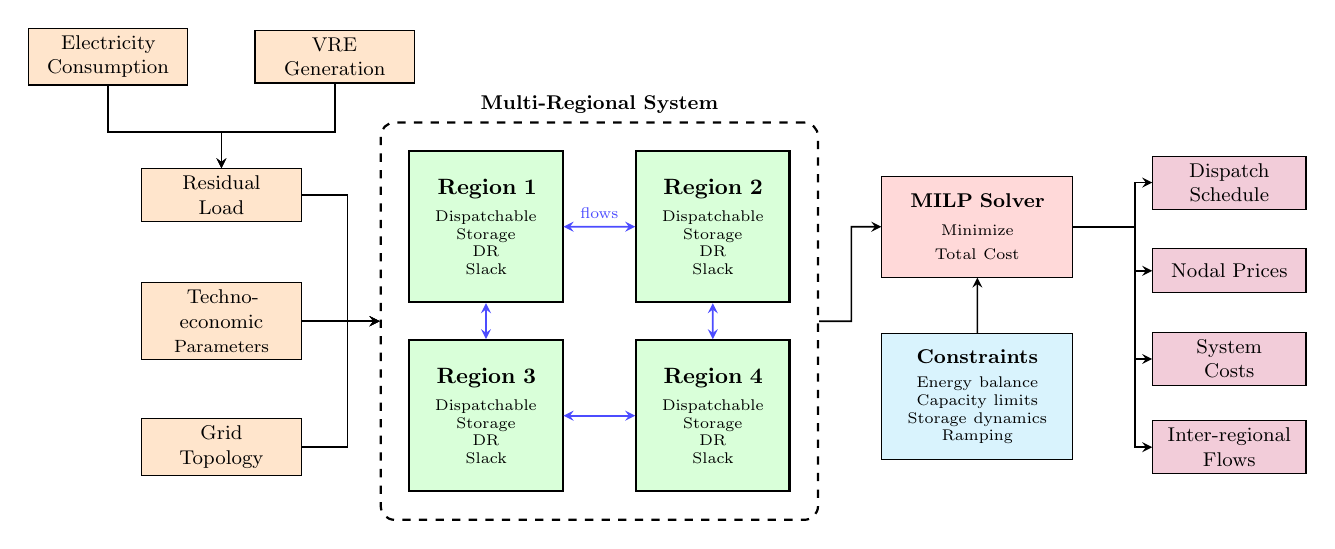
\begin{tikzpicture}[scale=0.8, transform shape,
    node distance=1.8cm and 2cm,
    box/.style={rectangle, draw, fill=blue!10, text width=2.6cm, align=center, minimum height=1.1cm, font=\small},
    region/.style={rectangle, draw, fill=green!15, text width=2.2cm, align=center, minimum height=2.4cm, thick},
    input/.style={rectangle, draw, fill=orange!20, text width=2.3cm, align=center, minimum height=0.7cm, font=\small},
    output/.style={rectangle, draw, fill=purple!20, text width=2.2cm, align=center, minimum height=0.7cm, font=\small},
    arrow/.style={->, >=stealth, semithick},
    exchange/.style={<->, >=stealth, semithick, blue!70}
]

\node[input] (consum) at (-7.8,6.2) {Electricity\\Consumption};
\node[input] (vre) at (-4.2,6.2) {VRE\\Generation};

% Input data (left side with more vertical spacing)
\node[input] (demand) at (-6,4) {Residual\\Load\\[0.05cm]};
\node[input] (params) at (-6,2) {Techno-\\economic\\[0.05cm]\footnotesize Parameters\\};
\node[input] (topology) at (-6,0) {Grid\\Topology\\};

% Four regions in a 2x2 grid (more spaced)
\node[region] (ara) at (-1.8,3.5) {\textbf{Region 1}\\[0.15cm]
    \scriptsize Dispatchable\\
    \scriptsize Storage\\
    \scriptsize DR\\
    \scriptsize Slack\\};
\node[region] (paca) at (1.8,3.5) {\textbf{Region 2}\\[0.15cm]
    \scriptsize Dispatchable\\
    \scriptsize Storage\\
    \scriptsize DR\\
    \scriptsize Slack\\};
\node[region] (occ) at (-1.8,0.5) {\textbf{Region 3}\\[0.15cm]
    \scriptsize Dispatchable\\
    \scriptsize Storage\\
    \scriptsize DR\\
    \scriptsize Slack\\};
\node[region] (naq) at (1.8,0.5) {\textbf{Region 4}\\[0.15cm]
    \scriptsize Dispatchable\\
    \scriptsize Storage\\
    \scriptsize DR\\
    \scriptsize Slack\\};
% Dashed box around all four regions with label
\node[draw, dashed, thick, rounded corners=5pt, fit=(ara) (paca) (occ) (naq), inner sep=10pt, fill=none, label={[font=\small\bfseries]above:Multi-Regional System}] (multi) {};


% Inter-regional exchanges (cleaner, fewer labels)
\draw[exchange] (ara) -- node[above, font=\scriptsize] {flows} (paca);
\draw[exchange] (ara) -- (occ);
\draw[exchange] (paca) -- (naq);
\draw[exchange] (occ) -- (naq);

% MILP Optimization block (right side)
\node[box, fill=red!15, text width=2.8cm, minimum height=1.6cm] (milp) at (6,3.5) {%
    \textbf{MILP Solver}\\[0.15cm]
    \scriptsize Minimize\\
    \scriptsize Total Cost};

% Constraints (below MILP)
\node[box, fill=cyan!15, text width=2.8cm, minimum height=2cm] (constraints) at (6,0.8) {%
    \textbf{Constraints}\\[0.1cm]
    \scriptsize Energy balance\\
    \scriptsize Capacity limits\\
    \scriptsize Storage dynamics\\
    \scriptsize Ramping\\};

% Outputs (right side with more spacing)
\node[output] (schedule) at (10,4.2) {Dispatch\\Schedule};
\node[output] (prices) at (10,2.8) {Nodal Prices\\[0.05cm]};
\node[output] (costs) at (10,1.4) {System\\Costs};
\node[output] (flows) at (10,0) {Inter-regional\\Flows};

\draw[arrow] (consum) |- (-5, 5) -| (demand);
\draw[arrow] (vre) |- (-5, 5) -| (demand);

% Arrows from inputs to regions (simplified)
\draw[arrow] (demand) -| (-4.0,2) |- (multi);
\draw[arrow] (params) -| (-4.0,2) |- (multi);
\draw[arrow] (topology) -| (-4.0,2) |- (multi);

% Arrows from regions to MILP
\draw[arrow] (multi.east) -- (4,2) |- (milp.west);

% Arrow from constraints to MILP
\draw[arrow] (constraints) -- (milp);

% Arrows from MILP to outputs
\draw[arrow] (milp) -| (8.5,4.2) |- (schedule);
\draw[arrow] (milp) -| (8.5,2.8) |- (prices);
\draw[arrow] (milp) -| (8.5,1.4) |- (costs);
\draw[arrow] (milp) -| (8.5,0) |- (flows);

\end{tikzpicture}

\caption{Schematic overview of the \textsc{RegionalFlex} multi-regional optimization methodology. The framework co-optimizes flexibility resources across four regions to meet residual load while minimizing total system cost.}
\label{fig:methodology_diagram}
\end{figure}

%--------------------------------------------------------
\subsection{Decision Variables and Cost Parameters}
\label{sec:variables}

\paragraph{}
Let $\mathcal{R}$ denote the set of regions and $\mathcal{T}$ the time index (e.g., half-hourly time steps). For each $(r,t) \in \mathcal{R} \times \mathcal{T}$, the following variables are defined:

\begin{table}[H]
\centering
\label{tab:variables}
\setlength{\tabcolsep}{6pt}
\renewcommand{\arraystretch}{1.25}

\newcolumntype{P}[1]{>{\RaggedRight\arraybackslash}p{#1}}
\newcolumntype{Z}{>{\RaggedRight\arraybackslash}X}

\begin{tabularx}{\linewidth}{@{}
l
P{0.24\linewidth}   % <-- reduced Meaning column
P{0.16\linewidth}
P{0.18\linewidth}
Z
@{}}
\toprule
\textbf{Symbol} &
\textbf{Meaning} &
\textbf{Domain} &
\textbf{Cost} &
\textbf{Cost value(s)} \\
\midrule

$g^{r,t}_k$
& Generation of technology $k$ in region $r$
& $g^{r,t}_k \ge 0$
& Marginal cost $C^r_k$ (€/MWh)
& Hydro: 20--25; Nuclear: 30; Gas: 75; Fuel: 85; Bio-fuel: 70 \\

\addlinespace
$u^{r,t}_k$
& Unit-commitment status of unit $k$
& $u^{r,t}_k \in \{0,1\}$
& Fixed cost $C^{\text{fixed}}_k$ (€/h)
& 100--210 \\

\addlinespace
$s^{r,t}_k$
& Startup indicator for unit $k$
& $s^{r,t}_k \in \{0,1\}$
& Startup cost $C^{\text{start}}_k$ (€/start)
& 200--1100 \\

\addlinespace
$c^{r,t}_s$
& Charging power of storage $s$
& $0 \le c^{r,t}_s \le P^{\max}_s$
& Charging cost $C^{\text{ch}}_s$ (€/MWh)
& 35 \\

\addlinespace
$d^{r,t}_s$
& Discharging power of storage $s$
& $0 \le d^{r,t}_s \le P^{\max}_s$
& Discharging cost $C^{\text{dis}}_s$ (€/MWh)
& 50 \\

\addlinespace
$soc^{r,t}_s$
& State of charge of storage $s$
& $0 \le soc^{r,t}_s \le SOC^{\max}_s$
& \shortstack{Efficiencies}
& $\eta^{\text{ch}}_s = 90\%$; $\eta^{\text{dis}}_s = 85$--90\%; $\delta_s = 0.808$ h \\


\addlinespace
$dr^{r,t}$
& Demand response (load reduction, with rebound recovery $\beta$)
& $0 \le dr^{r,t} \le \alpha_r RL^{r,t}$
& Marginal cost $C^{\text{DR}}$ (€/MWh)
& 120 \\
\addlinespace
$\beta,\,H_w=24$
& DR recovery share; DR recovery horizon
& $\beta \in [0,1]$
& --
& --\\

\addlinespace
$\overline{H}^{r,t}$
& Dispatchable-hydro availability cap (historical)
& $g^{r,t}_{\text{hydro}} \le \overline{H}^{r,t}$
& --
& -- \\

\addlinespace
$f^{r\rightarrow r',t}$
& Power flow from region $r$ to $r'$
& $0 \le f^{r\rightarrow r',t} \le F^{\max}_{r\to r'}$
& Flow cost $C^{\text{flow}}_{r\to r'}$ (€/MWh)
& 35; losses 0.025\%/km \\

\addlinespace
$slack^{r,t}_{\pm}$
& Positive / negative slack variables
& $slack^{r,t}_{\pm} \ge 0$
& Penalty $P^{\text{slack}}$ (€/MWh)
& 50\,000 \\

\bottomrule
\end{tabularx}
\caption{Decision variables, domains, and associated cost parameters used in the 2022 baseline configuration. Values are sourced according to the elements given in Section \ref{subsec:data}}
\end{table}




%--------------------------------------------------------



\label{sec:model}

The objective is to minimize the total system cost denoted as :

%--------------------------------------------------------------
\begin{equation}\label{eq:C0}
\min\;
\sum_{r,t}
\left[
\begin{aligned}
&\underbrace{\sum_k\!\left(C^r_k g^{r,t}_k
                 + C^{\text{fixed}}_k u^{r,t}_k
                 + C^{\text{start}}_k s^{r,t}_k\right)}_{\text{dispatchable generation}}
\\[4pt]
&\quad+\;
\underbrace{\sum_s\!\left(C^{\text{ch}}_s c^{r,t}_s
                 + C^{\text{dis}}_s d^{r,t}_s\right)}_{\text{storage}}
\\[4pt]
&\quad+\;
\underbrace{C^{\text{DR}}\,dr^{r,t}}_{\text{demand response}}
\\[4pt]
&\quad+\;
\underbrace{\sum_{r'\neq r} C^{\text{flow}}_{r\to r'}\,f^{r\to r',t}}_{\text{inter-regional exchanges}}
\\[4pt]
&\quad+\;
\underbrace{P^{\text{slack}}\bigl(slack^{r,t}_{+}+slack^{r,t}_{-}\bigr)}_{\text{adjustment terms}}
\end{aligned}
\right]
\end{equation}
%--------------------------------------------------------------




\subsection{Constraints}

\paragraph{}
The model includes:

\paragraph{C1. Energy balance (per region and timestep), following Kirchhoff's law:}
\begin{equation}\label{eq:C1}
\begin{split}
\sum_k g^{r,t}_k
  + \sum_s d^{r,t}_s
  + \sum_{r'\neq r} (1-\ell_{r'\to r})\, f^{r'\to r,t}
= RL^{r,t}
  + \sum_s c^{r,t}_s
  - dr^{r,t}
  + slack^{r,t}_{+}
  - slack^{r,t}_{-}
\end{split}
\end{equation}
\paragraph{}
The right-hand side is expressed in terms of the regional \emph{residual load} $RL^{r,t}$, defined as gross demand net of all non-dispatchable, must-run renewable injection. In addition to wind and solar, this explicitly includes run-of-river (RoR) hydro, which is governed by river inflows rather than by economic dispatch:
\begin{equation}\label{eq:residual_load}
RL^{r,t} = D^{r,t} - g^{r,t}_{\text{solar}} - g^{r,t}_{\text{wind}} - g^{r,t}_{\text{RoR}} .
\end{equation}
Netting RoR into the residual load (rather than treating it as a dispatchable resource) ensures that only the genuinely controllable share of hydro competes in the merit order, and prevents the model from crediting run-of-river output with flexibility it does not physically provide.

%---------------------------------------------------------------
% C2 – Generation capacity and UC linkage
%---------------------------------------------------------------
\paragraph{C2. Generation capacity and Unit Commitment (UC) linkage:}
\begin{subequations}\label{eq:C2}
\begin{alignat}{4}
0 &\le g^{r,t}_k \le G^{r}_k
   &\quad&\text{(name‑plate capacity)}  &\tag{3a}\label{eq:C2a}\\[4pt]
g^{r,t}_k &\le G^{r}_k\,u^{r,t}_k
         &\quad&\text{(output only if unit is ON)} &\tag{3b}\label{eq:C2b}\\[4pt]
s^{r,t}_k &\ge u^{r,t}_k - u^{r,t-1}_k
         &\quad&\text{(startup flag)}             &\tag{3c}\label{eq:C2c}\\[4pt]
u^{r,\tau}_k &\ge s^{r,t}_k,\;
   \tau=t,\dots,t+T^{\min\uparrow}_k-1
         &\quad&\text{(min‑up time)}              &\tag{3d}\label{eq:C2d}
\end{alignat}
\end{subequations}

%---------------------------------------------------------------
% C3 – Storage dynamics and bounds
%---------------------------------------------------------------
\paragraph{C3. Storage dynamics and bounds:}
\begin{subequations}\label{eq:C3}
\begin{alignat}{4}
\text{SOC}^{\,r,t+1}_s \;&=\;
   \text{SOC}^{\,r,t}_s\,\delta_s
   + \eta^{\text{ch}}_s\,c^{r,t}_s
   - \dfrac{1}{\eta^{\text{dis}}_s}\,d^{r,t}_s
   \quad&\hfill&\text{(energy balance)}       &\tag{4a}\label{eq:C3a}\\[6pt]
0 &\le \text{SOC}^{\,r,t}_s \le \text{SOC}^{\max}_s
   \quad&\hfill&\text{(storage capacity)}     &\tag{4b}\label{eq:C3b}\\[6pt]
0 &\le c^{r,t}_s \le P^{\max}_s, \qquad
   0 \le d^{r,t}_s \le P^{\max}_s
   \quad&\hfill&\text{(charge / discharge limits)} &\tag{4c}\label{eq:C3c}
\end{alignat}
\end{subequations}
\paragraph{}
These constraints describe the intertemporal dynamics of storage units by jointly limiting their instantaneous power (MW) and their energy content (MWh). The set of storage units in each region is $\mathcal{S}=\{\text{STEP},\,\text{batteries}\}$, comprising pumped-hydro storage (STEP) and electrochemical batteries, which differ in their power and energy ratings and round-trip efficiencies ($\eta^{\text{ch}}_s\eta^{\text{dis}}_s$); pumped-hydro storage is modelled here as a dedicated storage device through~\eqref{eq:C3} and is therefore distinct from, and not double-counted with, the dispatchable reservoir hydro of \eqref{eq:C7}. The power balance equation~\eqref{eq:C3a} enforces the energy balance of each storage device, accounting for charging and discharging efficiencies as well as standing losses, while the storage capacity inequality \eqref{eq:C3b} and the charge/discharge inequalities \eqref{eq:C3c} bound, respectively, the maximum energy that can be stored and the maximum power that can be injected or withdrawn at each time step. All together, these constraints ensure that storage contributes to system flexibility through temporally coupled energy shifting, rather than instantaneous load reduction.




\paragraph{C4. DR potential and rebound (payback):}
\begin{subequations}\label{eq:C4}
\begin{alignat}{2}
0 &\le dr^{r,t} \le \alpha_r\, RL^{r,t}
   &\qquad&\text{(hourly activation ceiling)} \label{eq:C4a}\\[4pt]
\sum_{\tau = t+1}^{t+H_w} \!\! rec^{r,\tau}_{t}
  &= \beta\, dr^{r,t}
   &\qquad&\text{(recovery / rebound)} \label{eq:C4b}
\end{alignat}
\end{subequations}
\paragraph{}
Earlier versions of the model represented demand response as \emph{pure load shedding}: curtailed consumption was permanently lost and never shifted to later periods. This is an optimistic assumption, since it grants DR an energy-reduction value that real, comfort-preserving demand-side programmes rarely deliver. We therefore introduce an explicit \emph{rebound} (payback) effect: a fraction $\beta$ of the energy shed at time $t$ is recovered as additional load over a subsequent horizon $H_w$ through the recovery terms $rec^{r,\tau}_{t}$, which re-enter the energy balance \eqref{eq:C1} as added demand. The parameter $\beta$ spans the full range of demand-side behaviour: $\beta = 0$ reproduces the previous pure-shedding assumption (energy is permanently curtailed), $\beta = 1$ corresponds to an energy-neutral load \emph{shift} (all shed energy is paid back), and the baseline adopts $\beta = 0.5$ with $H_w = \SI{24}{h}$. Because recovery is carried across successive optimization windows, this formulation captures the temporal coupling that distinguishes genuine load shifting from costless curtailment.


\paragraph{C5. Inter-regional flows:}
\begin{equation}
0 \le f^{r \rightarrow r',t} \le F^{\max}_{r \rightarrow r'}
\end{equation}
\paragraph{}
This constraint limits inter-regional electricity exchanges by the physical capacity of the transmission grid. Inter-regional flows are therefore constrained by existing transmission infrastructure, which was primarily designed to mesh the national territory. By explicitly modeling these capacity limits, the framework adopts an original perspective on the transmission grid: it evaluates a novel use of existing high-voltage assets for regional balancing.
\paragraph{}
This formulation adopts a transport (``pipe-and-bubble'', or net-transfer-capacity) representation of the grid: each corridor is bounded by an aggregate transfer limit, but voltage magnitudes, reactive power, and Kirchhoff's voltage law are not represented. A linearized DC power-flow model would instead redistribute injections across all parallel paths according to power-transfer distribution factors (PTDFs), and could therefore alter feasibility and loading on individual corridors. The aggregated four-region (single-node-per-region) representation adopted here is a deliberate scoping choice that keeps the multi-regional coordination problem tractable while preserving the dominant inter-regional balancing patterns; its implications are discussed among the limitations in \cref{sec:conclusions}.


\paragraph{C6. Ramping constraints:}
\begin{equation}
\bigl|\, g^{r,t}_k - g^{r,t-1}_k \,\bigr| \le \rho_k\, G^{r}_k
\end{equation}
\paragraph{}
This constraint captures the limited operational flexibility of dispatchable generation units by restricting the rate at which their output can be adjusted over time. It assumes that the generation of each unit can only increase or decrease by a given fraction of its installed capacity from one time step to the next, reflecting physical ramping limits and operational constraints. By bounding short-term variations in output, this formulation prevents unrealistically fast adjustments and ensures that flexibility is provided through feasible intertemporal trajectories rather than instantaneous re-dispatch. However, this static ramping limit represents a simplification compared to actual threshold-based ramping capabilities of power plants.

\paragraph{C7. Dispatchable-hydro availability cap:}
\begin{equation}\label{eq:C7}
g^{r,t}_{\text{hydro}} \le \overline{H}^{r,t},
\qquad
\overline{H}^{r,t} = \min\!\Big( H^{r,t}_{\text{obs}} - g^{r,t}_{\text{RoR}},\; \overline{P}^{\,r}_{\text{res}} \Big).
\end{equation}
\paragraph{}
A recurrent criticism of aggregated flexibility models is that hydro is treated as ``fully dispatchable up to nameplate capacity'', which mechanically inflates its contribution and ignores the energy and inflow limits of reservoirs. To address this, dispatchable (reservoir and pondage) hydro is bounded at each time step by an \emph{empirical availability cap} $\overline{H}^{r,t}$, defined as the same-year observed regional hydro production net of run-of-river, and additionally capped by the regional reservoir (lake) nameplate $\overline{P}^{\,r}_{\text{res}}$ reported in the ODR\'E register. This imposes a time-varying energy/availability budget that reflects seasonal inflows, reservoir levels, and competing water uses, so that hydro can provide flexibility only within its historically observed operating envelope rather than up to its full installed power. The structural importance of this single constraint is quantified in the robustness analysis of \cref{subsec:robust_hydro}.

\subsection{Dual Variables and LP Relaxation}

\paragraph{}
After solving the MILP, we freeze $\mathbf{y} = \mathbf{y}^\star$ and relax the integrality constraints to obtain a Linear Program. Solving the LP yields:

\begin{itemize}
  \item The dual variable $\boldsymbol{\lambda}_{r,t}$ associated with constraint~\eqref{eq:C1} represents the shadow price of the regional power balance, that is, the marginal value of an additional unit of electricity delivered in region $r$ at time $t$. In a setting where each region is modeled as a single node of the power system, this shadow price is naturally interpreted as a regional nodal price, reflecting the cost of the last flexibility resource activated locally.

  \item The dual variables $\boldsymbol{\mu}$ are associated with capacity constraints and capture the marginal value of relaxing physical limits, including inter-regional line flow capacities, storage charging and discharging power bounds, and DR activation ceilings. Economically, they reflect the scarcity of flexibility resources and quantify the shadow cost of capacity constraints that prevent additional power transfers or flexibility activation.

\end{itemize}

\paragraph{}
Because the integer commitment variables $\mathbf{y}$ are fixed before the LP relaxation, the prices $\lambda_{r,t}$ recovered here are restricted-LP marginal prices: they reflect the marginal generation, exchange, and flexibility cost of serving load, but they do \emph{not} internalize the start-up and no-load fixed costs of committed units. In a real market these non-convex costs would be settled through out-of-market uplift (make-whole) payments. An alternative such as Convex Hull Pricing \citep{gribik2007} would instead price the convex hull of the cost function, internalizing commitment costs directly and typically compressing the sharp scarcity spikes produced by binary commitment. We retain the restricted-LP convention for transparency and tractability; importantly, the \emph{ordering} of congestion value across corridors---which inter-regional links dominate and why---is driven by structural marginal-cost and capacity differentials and is therefore expected to be robust to the pricing convention, even though the absolute level of individual price spikes is not.



\subsection{Implementation}

\paragraph{}
The model is implemented in Python using \texttt{PuLP}. Constraints and cost parameters are dynamically built from a YAML configuration file, and post-processing scripts extract time-series of generation, DR, storage and inter-regional flows for visualization and comparison purposes.

\paragraph{}
The full year is solved as a sequence of overlapping rolling-horizon windows of 24 hours (48 half-hourly steps), which prevents the artificial anticipation of favourable storage-activation periods that would arise under perfect-foresight optimization over the whole year. State variables are handed over between successive windows: the end-of-window state of charge of each storage unit initializes the next window, and the demand-response recovery profile generated by \eqref{eq:C4b} is carried over so that rebound obligations incurred near a window boundary are honoured in the following window rather than discarded. The 2023 baseline (365 daily windows at half-hourly resolution, four regions) solves in approximately \SI{1770}{s} of wall-clock time (about \SI{100}{s} of model build and \SI{1430}{s} of solver time), while the 2022 case solves in roughly \SI{1560}{s}; runtime scales roughly linearly with the number of windows and is expected to grow with the number of regions and with finer spatial or temporal resolution, but remains well within reach for portability to other countries and generation mixes. Finally, across all reported runs the demand-imbalance slack variables $slack^{r,t}_{\pm}$ remain at zero, confirming that the baseline and all robustness scenarios are served without recourse to the high-penalty adjustment terms and are therefore strictly feasible.

\subsection{Data Sources}
\label{subsec:data}

\paragraph{}
The model relies on empirical data from publicly available platforms and national reports:

\begin{itemize}
  \item \textbf{Electricity demand} profiles are retrieved from the
        \emph{ODRÉ} platform\footnote{\url{https://opendata.reseaux-energies.fr}},
        which provides half-hourly regional consumption series for mainland France.
  \item \textbf{Renewable generation profiles} (solar and wind, half-hourly) also come from \emph{ODRÉ}.
  \item \textbf{Installed capacities} of dispatchable generation, run-of-river and reservoir hydro, and storage are taken from the regional registers of the French generation fleet published on \emph{ODRÉ} and in RTE's regional balance sheets. The storage fleet of each region is split into pumped-hydro storage (STEP) and batteries, whose regional power capacities are aggregated in Appendix~\ref{app:capacities}.
  \item \textbf{Techno-economic parameters} are estimated using a combination of institutional sources (RTE, ADEME, CRE, ENTSO-E, IEA) and peer-reviewed literature commonly used in power system optimization. In particular, generation cost assumptions rely on RTE’s reference balance sheet for the French power system \citep{rte2022fe2050}, complemented by international benchmarks from the IEA \citep{iea2020generation}. Storage efficiencies and operating characteristics are informed by expert and institutional reports from ADEME and the IEA \citep{ademe2024stockage_experts,iea_eces_2018}, as well as by the academic literature on the economics of electrical storage \citep{zerrahn2018economics}. Assumptions related to balancing and system flexibility are consistent with European market monitoring reports from ENTSO-E \citep{entsoe2020balancing}. Finally, reliability penalties are calibrated using the official French Value of Lost Load (VOLL) defined by the energy regulator \citep{cre2022voll}.

\end{itemize}

The study focuses on a strategic cluster of four interconnected regions:
Auvergne--Rh\^one--Alpes (ARA), Provence--Alpes--C\^ote d'Azur (PACA), Occitanie (OCC),
and Nouvelle--Aquitaine (NAQ). This selection is driven by the need to capture a
representative typology of energy mixes within a tractable multi-regional framework.
Rather than modeling the entire national grid, which would introduce redundancy
without necessarily adding methodological insight, these four regions were chosen
because they encompass the full spectrum of flexibility characteristics found in
the national system. The geographical location of the modeled regions and their
interconnections within the French transmission grid are illustrated in
\cref{fig:regions_map}. The four modeled regions are highlighted, together with the stylized inter-regional transmission links and regional production and storage capacities considered in the optimization model.

\begin{figure}[H]
  \centering
  \includegraphics[width=0.85\linewidth]{regionalflex_regions_map_2022.jpg}
  \caption{Geographical scope of the \textsc{RegionalFlex} tested framework.}
  \label{fig:regions_map}
\end{figure}



Specifically, these regions exhibit strongly contrasted profiles: ARA provides massive dispatchable hydro storage capabilities, PACA represents a "load-pocket" subject to transmission constraints with high solar potential, while Occitanie and Nouvelle-Aquitaine combine high shares of variable renewables (wind and solar) with nuclear baseload. This heterogeneity makes this cluster a comprehensive "test-bench" to analyze how regional coordination operates between zones with structurally different residual load patterns.

\paragraph{}
The baseline results reported below correspond to the operating year 2023, processed at a half-hourly resolution. The year 2023 is selected as the reference case because it combines observed weather-driven variability of variable renewable energies (VRE) and electricity demand with a restored, broadly normal availability of the existing French generation fleet, after the exceptional disturbances of the preceding year. To test the sensitivity of our conclusions to inter-annual conditions, we additionally re-solve the model for the year 2022 as part of the robustness analysis (\cref{subsec:robust_interannual}).

It is important to note that 2022 constitutes a particular year for the French electricity system. It was marked by the European gas crisis, reduced nuclear availability, and behavioural adjustments in electricity demand linked to the sharp increase in electricity prices. Contrasting 2023 with 2022 therefore provides a natural inter-annual stress test: it allows us to verify that the structural mechanisms captured by the model---the merit-order dispatch logic and the regional distribution of generation capacities---are not an artefact of the crisis year, while quantifying how a stressed year amplifies the economic value of flexibility.
Descriptive statistics of the regional residual load time series are provided in
\cref{app:residual_load}. Regional capacities and associated cost assumptions for each flexibility technology
are reported in \cref{app:capacities}, and transport capacities are reported in \cref{app:transport}.




% ----------------------------------------------------------------------------- 
%  Results section – RegionalFlex paper
% ----------------------------------------------------------------------------- 

\section{Results}\label{sec:results}
% All numbers refer to the 2023 base year unless stated otherwise.

%------------------------------------------------------------------
\subsection{A nuclear-dominant, low-carbon residual mix}\label{subsec:hydro_resilience}

\paragraph{}
Once variable renewables and run-of-river hydro have been netted out (\cref{eq:residual_load}), the residual load is met by an overwhelmingly low-carbon dispatchable mix. Nuclear baseload provides \SI{88.6}{\percent} of dispatchable generation, dispatchable (reservoir and pondage) hydro \SI{11.3}{\percent}, and thermal gas less than \SI{0.1}{\percent}; the total annual system cost is \EURM{8437} (\(\sim 8.4\)~G\texteuro). The modest share of hydro is a direct consequence of the empirical availability cap of \cref{eq:C7}: once dispatchable hydro is constrained to its same-year observed production envelope and reservoir nameplate, it can no longer act as a quasi-unlimited swing resource, and the bulk of the residual balancing falls to nuclear modulation. Because both nuclear and hydro are virtually zero-carbon at the point of dispatch and gas is marginal, the associated carbon intensity remains several orders of magnitude below French (\textasciitilde\SI{50}{g_{CO2}\,/kWh}) and European averages (\textasciitilde\SI{280}{g_{CO2}\,/kWh}). The mix is thus still almost fully decarbonised, but for a structurally different reason than previously reported: it is nuclear baseload, not hydro flexibility, that anchors the low-carbon outcome.

\paragraph{}
Seasonal dynamics are illustrated in \cref{fig:weekly_stack}, showing the weekly mean generation stack for the 2023 simulation year. Nuclear maintains a stable baseload throughout the year, while the now clearly separated run-of-river band follows river inflows and dispatchable (reservoir) hydro is confined to a narrow envelope around its historical availability. This separation makes explicit that the previously reported ``hydro backbone'' largely reflected uncapped reservoir output: when run-of-river is treated as must-run and reservoir hydro is energy-constrained, hydro's role contracts to targeted peaking and spatial balancing rather than bulk energy supply.

\begin{figure}[H]
  \centering
  
\includegraphics[width=\linewidth]{fig2b_weekly_stack_renewables.png}
  \caption[Weekly generation stack]{Weekly mean generation stack in \textsc{RegionalFlex} for the year 2023, with run-of-river shown as a distinct must-run band and dispatchable reservoir hydro (\emph{Hydro\_reservoir}) capped by its historical availability.}
  \label{fig:weekly_stack}
\end{figure}

\paragraph{}
To complement this seasonal view with the intraday operating logic, \cref{fig:rep_days} contrasts the system-aggregate generation stack on two representative days at the native half-hourly resolution: a high-demand winter weekday (Monday 23 January 2023, the peak-demand working day of the winter) and a low-demand summer public holiday (Tuesday 15 August 2023, Assumption Day). The two profiles confirm the structural picture of \cref{subsec:hydro_resilience} at the level of individual hours. On the winter weekday, total dispatch follows the characteristic twin-peak shape (a morning ramp and a pronounced evening peak above \SI{35}{GW}); nuclear supplies the bulk of the load as a near-flat baseload band, while capped reservoir hydro is dispatched precisely into the midday and evening peaks---visibly bulging exactly when residual load is highest---which is the targeted peaking and spatial-balancing role the availability cap is designed to enforce. Run-of-river contributes a steady must-run band, and solar and wind are minor in winter. On the summer holiday, total dispatch is roughly half as large (\(\sim\)\SI{17}{--}\SI{24}{GW}) and far flatter, reflecting the absence of industrial and commercial load; a large midday solar band displaces a substantial part of conventional generation, nuclear modulates downward, and both reservoir hydro and gas are barely called. On neither day do storage discharge or demand response contribute appreciably, consistent with their negligible baseline activation (\cref{subsec:dr_vs_storage}).

\begin{figure}[H]
  \centering
  \includegraphics[width=\linewidth]{fig_representative_days_2023.png}
  \caption[Representative-day generation stacks]{System-aggregate half-hourly generation stack for two representative days of 2023: \textbf{(a)} a high-demand winter weekday (Monday 23 January) and \textbf{(b)} a low-demand summer public holiday (Tuesday 15 August, Assumption Day). Coloured bands stack must-run renewables (solar, wind, run-of-river) and dispatchable generation (capped reservoir hydro, nuclear, thermal gas/fuel, biofuel). Inter-regional flows net out at the system-aggregate level.}
  \label{fig:rep_days}
\end{figure}

%------------------------------------------------------------------
\subsection{Demand response and storage are marginal at baseline}
\label{subsec:dr_vs_storage}

\paragraph{}
A central---and initially counter-intuitive---baseline result is that the two ``classic'' local flexibility instruments, demand response and storage, are barely activated. Under the baseline configuration ($\beta = 0.5$, capped hydro), demand response contributes \SI{0}{GWh}: with a realistic rebound effect, shedding load merely defers it, and the deferred consumption must be re-served within a day at a comparable or higher marginal cost, so shed-only DR is never economically dispatched. Storage is likewise negligible, with an annual discharge of about \SI{57}{GWh}---roughly \SI{0.03}{\percent} of demand---against an installed pumped-hydro capacity orders of magnitude larger. Instead, short-term residual balancing is provided almost entirely by nuclear modulation within its ramping envelope and by inter-regional exchanges (\cref{subsec:regional_trading}).

\paragraph{}
The reason storage barely cycles is structural rather than a matter of narrow price spreads. Let $p_t$ denote the regional nodal price, $\eta_{\mathrm{rt}}\in(0,1)$ the round-trip efficiency, and $c_{\mathrm{var}}$ the variable cycling cost (O\&M, degradation, self-discharge). A profitable cycle requires
\begin{equation}
  p_t-\frac{p_{\tau}}{\eta_{\mathrm{rt}}}\ge c_{\mathrm{var}},
  \label{eq:spread_condition}
\end{equation}
i.e. a sufficiently high price at the discharge hour $t$ relative to the charge hour $\tau$. In the nuclear-dominated 2023 mix, nodal prices sit at the low, flat nuclear marginal cost for the overwhelming majority of hours, and rise sharply only during rare scarcity events. Once nuclear ramping is correctly represented, these scarcity spikes largely disappear: both charge and discharge occur at near-flat, nuclear-marginal prices (energy-weighted \(\approx\)~\SI{56}{\EUR/\MWh} on both sides), so condition~\eqref{eq:spread_condition} is almost never profitable and total throughput stays around \SI{57}{GWh} (\(\sim\)\SI{0.03}{\percent} of demand). Storage thus provides negligible arbitrage value in the nuclear-dominated 2023 mix rather than acting as a routine balancing resource.

\paragraph{}
It is precisely this baseline that overturns the headline finding of earlier formulations, where demand response appeared to dominate storage by nearly two orders of magnitude. That result was an artefact of two optimistic assumptions acting together: uncapped hydro suppressed the need for any local flexibility, while pure-shedding DR (no rebound) let the optimizer curtail load at no intertemporal cost. We therefore do not report a baseline DR-versus-storage ranking; instead, \cref{subsec:robust_dr} shows that demand response remains structurally marginal regardless of the rebound assumption, because its activation cost exceeds the marginal cost of every available generation and exchange option once nuclear ramping is correctly represented. The regional nodal price used throughout represents an average regional cost of flexibility; local market effects and consumer incentives lie beyond this paper's scope.

%------------------------------------------------------------------
\subsection{Inter-regional exchanges as the primary flexibility channel}
\label{subsec:regional_trading}

\paragraph{}
With hydro energy-constrained and DR and storage inactive at baseline, inter-regional exchanges become the dominant flexibility instrument. Annual directed exchanges reach \SI{30.6}{TWh}, equivalent to about \SI{17}{\percent} of regional demand---no longer a marginal contribution but the principal mechanism through which the four regions balance their residual load. Flows run predominantly westward-to-southeast, from the renewable- and nuclear-rich Atlantic and central regions toward the import-dependent Provence--Alpes--Côte~d'Azur (PACA) load pocket, and generate substantial economic value for grid operators.

\paragraph{}
In our framework, congestion revenues quantify this grid value.
They arise whenever nodal (regional) prices differ between connected regions,
reflecting transmission constraints and marginal cost differentials.
For each directed interconnection $i \to j$ and time step~$t$,
the congestion rent is defined as
\begin{equation}
  CR_{i \to j}(t) = F_{i \to j}(t)\, \big(P_j(t) - P_i(t)\big),
\end{equation}
where $F_{i \to j}(t)$ denotes the inter-regional power flow (MW),
and $P_i(t),P_j(t)$ are the regional nodal prices (€/MWh).
Since the optimization runs at 30-minute resolution, energy volumes are obtained by
multiplying flows by~0.5, so that $F_{i \to j}(t)\!\times\!0.5$ corresponds to MWh.
Total annual congestion rents are then computed as
\begin{equation}
  CR^{\text{tot}} = \sum_{t,i,j} CR_{i \to j}(t)\times0.5.
\end{equation}

\paragraph{}
Applying this formulation to the full-year 2023 simulation yields total annual congestion rents of approximately \SI{905}{\MEUR}---nearly eight times the value obtained under the uncapped-hydro formulation (\cref{subsec:robust_hydro}), reflecting the larger and more persistent price differentials of a nuclear-anchored, exchange-dependent system. The dominant contribution comes from the ARA$\to$PACA corridor (\SI{691}{\MEUR}), which carries low-cost nuclear and hydro energy from Auvergne--Rhône--Alpes (average nodal price \(\approx\)~\SI{30}{\EUR/\MWh}) into the structurally short PACA load pocket (\(\approx\)~\SI{60}{\EUR/\MWh}). The OCC$\to$PACA corridor adds \SI{152}{\MEUR} and ARA$\to$OCC \SI{58}{\MEUR}, while all remaining directed links are negligible. All three dominant corridors correspond to physical inter-regional lines in the network (\cref{app:transport}), so the rents map directly onto real transfer capability feeding the PACA load pocket.

\begin{table}[h]
  \centering
  \begin{tabular}{l r}
  \hline
  Interconnection & Congestion rent (M€) \\
  \hline
  ARA $\to$ PACA & 690.9 \\
  OCC $\to$ PACA & 152.3 \\
  ARA $\to$ OCC  & 58.0 \\
  NAQ $\to$ OCC  & 4.1 \\
  Other links    & $<1$ \\
  \hline
  \textbf{Total} & \textbf{905.4} \\
  \hline
  \end{tabular}
  \caption{Annual directed congestion rents by interconnection in the 2023 baseline (in million €). Values are summed over directed half-hourly flows; reverse-direction and minor links contribute less than \SI{1}{\MEUR} each.}
  \label{tab:congestion_rents}
\end{table}

\paragraph{}
Congestion rents thus reflect the spatial value of flexibility: they capture how grid operators (TSOs) monetize price differentials between regions by enabling energy reallocation. In the 2023 mix these differentials are driven mainly by the spatial mismatch between low-cost nuclear and renewable supply in the western and central regions and the structural import dependence of PACA, whose limited internal flexibility (no nuclear, capped hydro) leaves it reliant on imports during scarcity hours. Inter-regional flows relieve this locational scarcity and generate the observed rents, confirming that the regional nodal price used here corresponds to a \emph{technical system price}---a shadow value of inter-regional flexibility.

\paragraph{}
Overall, inter-regional exchanges have moved from a marginal contributor to the system's primary flexibility channel (\(\sim\)\SI{17}{\percent} of demand) while yielding substantial economic value (\(\sim\)\SI{905}{\MEUR}). These congestion rents also provide an economic signal for transmission capacity investment: the persistent and highly concentrated price differential on the corridors feeding PACA reveals precisely where additional inter-regional transfer capability would yield the highest system-wide benefits.

%------------------------------------------------------------------
%------------------------------------------------------------------
%------------------------------------------------------------------
\subsection{Ramping adequacy and probabilistic flexibility metrics}
\label{subsec:irre_efs_results}

\paragraph{}
To complement energy and cost-based indicators, we evaluate the
\emph{ramping adequacy} of the system using the probabilistic metrics
introduced by \citet{abdin2018integrated,abdin2019resilient}:
the \emph{Insufficient Ramping Resource Expectation} (\textsc{IRRE})
and the \emph{Expected Flexibility Shortfall} (\textsc{EFS}).
These indicators jointly measure the frequency (\textsc{IRRE}) and the
average magnitude (\textsc{EFS}) of ramping shortages when the net load
variation $\Delta RL(t)$ exceeds the available ramping
capability $R^{\pm}(t)$.

\paragraph{}
For each region, upward and downward ramping headrooms, $R_r^{+}(t)$ and $R_r^{-}(t)$,
are derived dynamically from generation, storage, and demand-response
constraints.
Shortage events occur whenever
$\pm\Delta RL_r(t)>R^{\pm}_r(t)$.
The corresponding indicators are defined as:
\begin{align}
\text{IRRE}^{\pm}_r &=
\frac{1}{T}\sum_t
\mathds{1}\!\left(
  \pm\Delta RL_r(t)
  > R^{\pm}_r(t)
\right),
\\[4pt]
\text{EFS}^{\pm}_r &=
\mathbb{E}\!\left[
  \pm\bigl(\Delta  RL_r(t)-R^{\pm}_r(t)\bigr)
  \;\middle|\;
  \pm\Delta RL_r(t)>R^{\pm}_r(t)
\right].
\end{align}

\paragraph{}
Table~\ref{tab:irre_efs_yaml} summarizes the regional and system-level
values obtained from the time-varying ramping simulation.
Two features stand out. First, \emph{upward} ramping is fully adequate: once
nuclear and reservoir hydro ramp within their realistic per-step envelopes, the
local dispatchable fleet always meets rising residual load, so \textsc{IRRE}$^{+}=0$
in every region. Second, the residual stress is \emph{downward} and spatially
concentrated: it is essentially absent in the generation-rich ARA and OCC but
appears in the import-dependent PACA (\SI{14.5}{\percent} of steps) and, marginally,
NAQ (\SI{1.0}{\percent}). These regions hold little local dispatchable generation
to curtail when residual load falls sharply, so the surplus must be exported rather
than absorbed in place---the mirror image of their import dependence during peaks.

\begin{table}[H]
\centering
\begin{tabular}{lrrrr}
\hline
Region & IRRE$^{+}$ (\%) & IRRE$^{-}$ (\%) &
EFS$^{+}$ (MW) & EFS$^{-}$ (MW) \\
\hline
ARA          &  0.00 &  0.00 & --    & --    \\
NAQ             &  0.00 &  0.97 & --    & 138.3 \\
OCC                       &  0.00 &  0.01 & --    &  42.9 \\
PACA    &  0.00 & 14.52 & --    &  87.7 \\
\hline
\textbf{System aggregate}       & \textbf{0.00} & \textbf{0.00} &
-- & -- \\
\hline
\end{tabular}
\caption[IRRE and EFS metrics (regional and system levels)]{Frequency
(IRRE) and conditional magnitude (EFS) of ramping shortages in
\textsc{RegionalFlex}, computed from time-varying ramping headrooms
derived from generation, storage and demand-response capabilities.}
\label{tab:irre_efs_yaml}
\end{table}

\paragraph{}
The results show that, with physically realistic ramp envelopes, local ramping
adequacy is no longer a binding concern on the upward side, and that the only
material stress---downward shortfalls in the import-dependent PACA load
pocket---is modest in magnitude (conditional \textsc{EFS}$^{-}$ below
\SI{140}{MW}). Most strikingly, when the four regions are pooled the
system-aggregate \textsc{IRRE} falls to zero in both directions: ramping
surpluses in the generation-rich regions exactly offset the local deficits of
PACA and NAQ at every half-hour. In other words, the residual ramping stress is
not a system-wide adequacy problem but a \emph{spatial allocation} problem that
inter-regional coordination resolves---the same mechanism that drives the
exchange flows and congestion rents of \cref{subsec:regional_trading}.
Following \citet{abdin2018integrated}, these indicators thus provide
a probabilistic and physically grounded view of flexibility adequacy,
confirming that regional pooling, rather than additional fast-ramping capacity,
is the binding lever for ramping adequacy in this system. The residual local
stress that remains reflects the four-region structure of the model: the limited
interconnection capacity feeding PACA constrains how quickly its downward surplus
can be exported. In a more finely interconnected setting---through additional
links or higher transfer capacities---this residual local \textsc{IRRE}$^{-}$
would be expected to shrink further, as neighbouring areas could absorb PACA's
downward surpluses even more readily.


%------------------------------------------------------------------
\subsection{Robustness analysis}
\label{subsec:robustness}

\paragraph{}
The baseline results above rest on two modelling choices that previous formulations treated very differently: the empirical hydro availability cap (\cref{eq:C7}) and the demand-response rebound parameter $\beta$ (\cref{eq:C4}). Because these choices reverse the qualitative ordering of flexibility instruments relative to earlier work, we subject them to a dedicated robustness battery, complemented by an inter-annual replication. All scenarios solve to optimality with zero slack activation.

\subsubsection{Sensitivity to the hydro energy budget}
\label{subsec:robust_hydro}

\paragraph{}
We compare the baseline (capped hydro) against a ``simplified hydro'' scenario that removes the availability cap and lets reservoir hydro dispatch freely up to nameplate capacity---the assumption implicit in the earlier version of the model. The contrast is stark (\cref{tab:robust_hydro}, \cref{fig:hydro_sens}): without the cap, hydro jumps from \SI{11.3}{\percent} to \SI{71.0}{\percent} of dispatchable generation and displaces nuclear, total system cost falls from \EURM{8437} to \EURM{5767}, and---because abundant local hydro removes the need to import---inter-regional exchanges collapse from \SI{30.6}{TWh} to \SI{4.1}{TWh} and congestion rents from \SI{905}{\MEUR} to \SI{117}{\MEUR}. The previously reported ``hydro is the backbone of regional flexibility'' result is therefore not a structural property of the system but an artefact of unconstrained hydro: once a realistic energy budget is imposed, the system reorganizes around nuclear baseload and inter-regional exchanges.

\begin{table}[H]
  \centering
  \begin{tabular}{lrr}
  \hline
  Indicator & Baseline (capped) & Simplified (uncapped) \\
  \hline
  Hydro share (\%)            & 11.3 & 71.0 \\
  Nuclear share (\%)          & 88.6 & 29.0 \\
  Total cost (M€)             & 8\,437 & 5\,767 \\
  Exchanges (TWh)             & 30.6 & 4.1  \\
  Congestion rents (M€)       & 905.4 & 116.6 \\
  \hline
  \end{tabular}
  \caption{Hydro energy-budget sensitivity: baseline (empirical availability cap) versus simplified (uncapped, fully dispatchable to nameplate).}
  \label{tab:robust_hydro}
\end{table}

\begin{figure}[H]
  \centering
  \includegraphics[width=0.8\linewidth]{hydro_sensitivity.png}
  \caption[Hydro sensitivity]{Dispatchable-generation shares under the capped (baseline) and uncapped (simplified) hydro assumptions.}
  \label{fig:hydro_sens}
\end{figure}

\subsubsection{Sensitivity to the demand-response rebound effect}
\label{subsec:robust_dr}

\paragraph{}
We next vary the rebound parameter $\beta \in \{0, 0.5, 1\}$, holding all else at the baseline. The result is unambiguous: demand response is \emph{never} dispatched, for any value of $\beta$. The three solves are numerically identical in every reported aggregate---zero DR activation, a total system cost of \EURM{8437}, directed exchanges of \SI{30.6}{TWh}, and congestion rents of \SI{905}{\MEUR}---so the rebound assumption has no bearing on the baseline outcome. The reason is purely economic: the demand-response activation cost (\SI{120}{\EUR/\MWh}) exceeds the marginal cost of every available generation and exchange option, including the most expensive thermal units (\(\le\)\SI{90}{\EUR/\MWh}), so shedding is dominated regardless of whether it carries a payback obligation. Demand response is therefore \emph{structurally} marginal in this system rather than contingent on the rebound parameterisation.

\paragraph{}
This result also retracts a finding of earlier formulations, where pure shedding ($\beta=0$) appeared to activate hundreds of GWh of demand response. That activation was an artefact of an over-tight nuclear ramping representation: when nuclear could not follow load, the optimizer substituted demand shedding for otherwise unserved energy. Once nuclear ramping is corrected, no such substitution is needed and demand response collapses to zero for all $\beta$, leaving inter-regional exchanges as the sole active short-term balancing channel.

\subsubsection{Inter-annual robustness (2022 vs.\ 2023)}
\label{subsec:robust_interannual}

\paragraph{}
Finally, we re-solve the full baseline for 2022---the European energy-crisis year---to check that the structural mechanism is not an artefact of the reference year (\cref{tab:robust_interannual}). Both years are strongly nuclear-dominated (nuclear share \SI{88.6}{\percent} in 2023 versus \SI{91.4}{\percent} in 2022) and exchange-driven, confirming that the qualitative picture is stable across very different weather and availability conditions. The crisis year is, as expected, more stressed: total cost rises to \EURM{9714} and congestion rents to \SI{1084}{\MEUR}, i.e.\ the value of inter-regional flexibility is \emph{amplified} under tight supply conditions---precisely the direction one would expect, and a useful caveat on the absolute magnitudes reported for any single year.

\begin{table}[H]
  \centering
  \begin{tabular}{lrr}
  \hline
  Indicator & 2023 (baseline) & 2022 (crisis year) \\
  \hline
  Nuclear share (\%)     & 88.6 & 91.4 \\
  Hydro share (\%)       & 11.3 & 8.1  \\
  Total cost (M€)        & 8\,437 & 9\,714 \\
  Exchanges (TWh)        & 30.6 & 35.5 \\
  Congestion rents (M€)  & 905.4 & 1\,084.4 \\
  \hline
  \end{tabular}
  \caption{Inter-annual robustness: baseline 2023 versus a 2022 re-solve under identical model settings.}
  \label{tab:robust_interannual}
\end{table}


% ----------------------------------------------------------------------------- 
%  End of results section
% ---------------------------------------------------------------------------


\section{Conclusions and Research Avenues}
\label{sec:conclusions}

This paper has introduced \textsc{RegionalFlex}, a multi-regional MILP framework 
that co-optimizes dispatchable generation, storage, demand response, and inter-regional 
exchanges to balance half-hourly residual load across four French regions, using the 
operating year 2023 as a baseline and 2022 as an inter-annual robustness check. 
By explicitly modelling residual load after VRE \emph{and} run-of-river injection, by 
constraining dispatchable hydro to its empirical availability budget, and by representing 
demand response with a load-recovery effect, the framework isolates the flexibility layer 
of the power system and quantifies how different instruments contribute to adequacy under 
realistic techno-economic constraints.

Around the flexibility tools aspect, four central findings emerge. First, the optimized residual mix is overwhelmingly 
low-carbon but \emph{nuclear-anchored} rather than hydro-anchored: nuclear baseload provides \SI{88.6}{\percent} 
of dispatchable generation, capped reservoir hydro \SI{11.3}{\percent}, and thermal gas less than \SI{0.1}{\percent}. 
Hydro is therefore not the backbone of regional flexibility; once held to its historical energy budget, it acts as a 
targeted peaking and spatial-balancing resource. Second, inter-regional exchanges are the system's primary flexibility 
channel, reaching \SI{30.6}{TWh} (\(\sim\)\SI{17}{\percent} of demand) and generating congestion rents of \(\sim 905\)~M\texteuro, 
highly concentrated on the physical corridors feeding the import-dependent Provence--Alpes--Côte d'Azur load pocket. Third, the local 
``classic'' instruments are marginal at baseline: storage cycles only \(\sim\)\SI{57}{GWh} (\(\sim\)\SI{0.03}{\percent} of demand) and demand response is not dispatched 
at all---and, unlike in earlier formulations, this marginality is \emph{structural}: demand response stays at zero for every value of the rebound 
parameter $\beta$ because its activation cost exceeds that of all available generation and exchange options. Fourth, probabilistic ramping 
metrics (IRRE/EFS) show that, once ramp limits are physically calibrated, upward ramping is fully adequate and the only residual 
stress is a modest \emph{downward} shortfall in the import-dependent Provence--Alpes--Côte d'Azur load pocket---which vanishes 
entirely at the system-aggregate level, confirming that regional pooling, not additional fast-ramping capacity, is the binding 
lever for ramping adequacy. Crucially, a dedicated robustness analysis 
confirms that these conclusions are driven by the modelling of hydro and DR rather than by the choice of year: the 
hydro-dominant outcome reappears only when the availability cap is removed, and the nuclear-and-exchange structure is stable 
across 2022 and 2023.

Consequently, the local activation and remuneration of flexibility resources do not merely affect short-term system operation, but may signal a deeper bifurcation in how power system flexibility is conceptualized, coordinated, and governed across spatial scales. The 
evidence of regional price differentials suggest that flexibility is not solely a local characteristic of end-use consumption but emerges from interactions across multiple spatial layers. In this sense, the results point out to the relevance of an intermediate regional tier for coordinating flexibility resources, enabling targeted exchanges, and revealing congestion-driven value through nodal shadow prices. These 
insights contribute to the broader discussion on whether increasing VRE shares 
necessitate a partial decentralisation of system operation---not by fragmenting 
national coordination, but by enriching it with regional decision layers.

\medskip

\noindent
\textsc{RegionalFlex} also produces dual variables associated with the regional 
energy-balance constraints. The resulting multipliers~$\lambda_{r,t}$ can be 
interpreted as \emph{technical nodal prices}, i.e., the marginal cost of serving an 
additional MWh of residual load in region~$r$ at time~$t$. A natural extension of this work is to compare the optimized operational cost with the hypothetical revenue that would be collected under regional nodal pricing. In this perspective, nodal revenues would be obtained by valuing regional residual load at time-varying regional nodal prices, thereby allowing an explicit assessment of the gap between physical system optimization and price-based remuneration.
Such a comparison would quantify infra-marginal rents associated with flexible 
technologies and congested lines, clarify how much of the total system cost could 
be covered by locational pricing, and help bridge the gap between planning-oriented and VRE-based optimization and real-world market design, in the context of the energy transition.

\medskip

At the same time, several modeling assumptions delimit the scope of inference. 
The geographical resolution---four large regions modelled as single nodes with a transport 
(net-transfer-capacity) representation and no explicit DC power-flow constraints---likely 
overestimates intra-regional pooling of flexibility and understates the role of internal 
and loop-flow congestion; the dominant inter-regional balancing patterns are nonetheless 
preserved. Two limitations that earlier versions shared have now been addressed directly in 
the baseline: dispatchable hydro is bounded by an empirical availability budget rather than 
treated as power-constrained to nameplate, and demand response carries an explicit rebound 
effect rather than being modelled as costless instantaneous shedding. The robustness analysis 
(\cref{subsec:robustness}) shows that these two refinements, far from being second-order, 
\emph{reverse} the qualitative ordering of flexibility instruments: there is no longer a fixed 
``hydro $\gg$ DR $\gg$ storage'' hierarchy, but rather a nuclear-and-exchange–dominated baseline 
in which the apparent value of hydro is highly sensitive to its modelling while demand response is robustly marginal. Storage is 
still represented through fixed capacities and exogenous cycling costs, which omits investment 
decisions and the coupling between long-term storage sizing and short-term dispatch.

\medskip

These limitations outline a coherent research agenda structured around four axes.
\emph{(i) hydro energy modelling.} The baseline now separates run-of-river (netted into residual load) from dispatchable reservoir hydro and bounds the latter by an empirical, same-year availability budget (\cref{eq:C7}). This resolves the most consequential limitation of the earlier version, but it remains a reduced-form representation: it does not model reservoir state, cascade hydraulics, inflow forecasts, or the inter-temporal value of stored water. A natural extension is an explicit reservoir-storage formulation with seasonal inflow series and water-value functions, which would refine hydro's peaking and spatial-balancing role beyond the historical envelope used here.
\emph{(ii) grid resolution and congestion modelling.} Because exchanges are now the system's primary flexibility channel, the transport representation of the grid becomes the most important remaining simplification. Extending 
\textsc{RegionalFlex} to a finer regional partition, richer interconnections---including 
cross-border links---and at least DC load-flow constraints (PTDF-based) would enable a more 
realistic assessment of congestion rents, spatial price formation, and ramping 
adequacy, and would test whether the highly concentrated corridor rents reported here survive a physically meshed representation. A further extension would adopt a Convex Hull Pricing scheme to internalize commitment costs and assess the robustness of the price-spike structure underlying the congestion rents. Increasing transfer capacities is expected to lower IRRE and EFS by allowing 
neighbouring ramping surpluses to compensate local deficits. 
\emph{(ii-bis) comparison with operational multi-regional systems.} The structural result that an intermediate regional tier carries substantial coordination value invites systematic comparison with power systems where such coordination is already operational---notably China's inter-provincial and inter-regional dispatch and trading mechanisms \citep{china_interprovincial,china_regional_dispatch}---to distinguish which benefits stem from regional coordination per se and which from the specific French context.
\emph{(iii) End-uses modelling of flexibility.} Refining DR into sheddable and 
shiftable components, including intertemporal recovery constraints and simple comfort 
or welfare metrics, would yield more realistic downward flexibility estimates and allow 
a welfare-based comparison with storage. Embedding storage in a capacity-expansion 
layer would similarly clarify the conditions under which different storage technologies 
complement or substitute demand-side measures. 
\emph{(iv) Multi-level governance of flexibility.} The results highlight the potential 
operational benefits of regional coordination, but regulatory and institutional aspects 
(TSO--DSO interactions, allocation of congestion revenues, compatibility with national 
and European market rules) remain unmodelled. Coupling \textsc{RegionalFlex} with 
multi-level regulatory designs would provide a richer answer to the motivating 
question: \emph{under what conditions does the energy transition require a 
reconfiguration of power-system governance around an intermediate regional tier?}


\section*{Data and code availability}

\noindent The \textsc{RegionalFlex} optimization model, the configuration files used to produce the 2023 baseline and all robustness scenarios, and the post-processing scripts that generate the figures and tables reported here will be made available in a public repository upon publication. All input data are derived from openly accessible sources: half-hourly regional consumption and renewable generation series from the ODR\'E platform (\url{https://opendata.reseaux-energies.fr}) and the national installed-capacity register, together with the techno-economic parameters documented in \cref{subsec:data} and the appendices.

\section*{Declaration of generative AI and AI-assisted technologies in the manuscript preparation process}

\noindent During the preparation of this work the authors used ChatGPT, Claude and Gemini in order to assist with coding and language editing from French. After using these tools/services, the authors reviewed and edited the content as needed and take full responsibility for the content of the published article.



\bibliography{references}

\appendix
\section{Descriptive statistics of regional residual load}\label{app:residual_load}

\begin{table}[H]
\centering
\label{tab:residual_load_stats}
\setlength{\tabcolsep}{6pt}
\renewcommand{\arraystretch}{1.25}
\begin{tabular}{lcccc}
\toprule
\textbf{Statistic} 
& \textbf{ARA} 
& \textbf{NAQ} 
& \textbf{OCC} 
& \textbf{PACA} \\
\midrule
Mean (MW)      & 4\,310 & 3\,194 & 2\,365 & 3\,457 \\
Standard deviation (MW) & 1\,341 & 1\,241 & 1\,123 &   876 \\
Minimum (MW)  & 1\,027 & $-$292 & $-$1\,847 & 1\,529 \\
Maximum (MW)  & 8\,929 & 7\,261 & 5\,990 & 6\,354 \\
\bottomrule
\end{tabular}
\caption{Descriptive statistics of regional residual load time series (2023).
Residual load is defined as electricity demand minus wind, solar, \emph{and} run-of-river hydro generation (\cref{eq:residual_load}). Negative minima in NAQ and OCC indicate hours of net renewable surplus.}
\end{table}


\section{Inter-regional transport capacities}\label{app:transport}

\begin{table}[H]
\centering
\setlength{\tabcolsep}{6pt}
\renewcommand{\arraystretch}{1.15}
\begin{tabularx}{\linewidth}{X X X X X}
\toprule
\textbf{From $\backslash$ To} & \textbf{ARA} & \textbf{PACA} & \textbf{OCC} & \textbf{NAQ} \\
\midrule
\textbf{ARA}  & --   & 5\,000 & 2\,750 & 500 \\
\textbf{PACA} & 5\,000 & --   & 1\,500 & 0 \\
\textbf{OCC}  & 2\,750 & 1\,500 & --   & 1\,750 \\
\textbf{NAQ}  & 500  & 0     & 1\,750 & -- \\
\bottomrule
\end{tabularx}

\vspace{2mm}
\caption{Aggregated inter-regional transport capacity limits (MW) used in the \textsc{RegionalFlex} model (2023 baseline; unchanged from 2022). A value of 0 indicates that no direct interconnection is represented between the two regions in the aggregated grid.}
\label{tab:transport_capacities}
\end{table}

\section{Regional flexibility capacities and costs}\label{app:capacities}

\begin{table}[H]
\centering
\setlength{\tabcolsep}{6pt}
\renewcommand{\arraystretch}{1}
\begin{tabularx}{\linewidth}{l X r r}
\toprule
\textbf{Region} & \textbf{Technology} & \textbf{Capacity (MW)} & \textbf{Cost (€/MWh)} \\
\midrule
\multirow{9}{*}{ARA}
& Hydro (nameplate)  & 11\,479  & 20  \\
& \quad reservoir cap $\overline{P}_{\text{res}}$ & 3\,329 & --  \\
& Nuclear            & 13\,570  & 30  \\
& Thermal gas        &   930    & 75  \\
& Thermal fuel       &   115    & 85  \\
& Biofuel            &   214    & 70  \\
& Storage (STEP+batt.)    & 3\,381   & 35 / 50  \\
& Demand response    & $5\% \cdot RL_{ARA,t}$ & 120  \\
\addlinespace
\multirow{9}{*}{PACA}
& Hydro (nameplate)  & 3\,264  & 20  \\
& \quad reservoir cap $\overline{P}_{\text{res}}$ & 1\,947 & --  \\
& Nuclear            & 0  & 30  \\
& Thermal gas        & 2\,363   & 75  \\
& Thermal fuel       &   362   & 85  \\
& Biofuel            &   398   & 70  \\
& Storage (STEP+batt.)    & 14     & 35 / 50  \\
& Demand response    & $5\% \cdot RL_{PACA,t}$ & 120 \\
\addlinespace
\multirow{9}{*}{OCC}
& Hydro (nameplate)  & 5\,411  & 25  \\
& \quad reservoir cap $\overline{P}_{\text{res}}$ & 2\,345 & --  \\
& Nuclear            & 2\,620  & 30  \\
& Thermal gas        &   186   & 75  \\
& Thermal fuel       &   149   & 85  \\
& Biofuel            &   178   & 70  \\
& Storage (STEP+batt.)    & 983  & 35 / 50  \\
& Demand response    & $5\% \cdot RL_{OCC,t}$ & 120 \\
\addlinespace
\multirow{9}{*}{NAQ}
& Hydro (nameplate)  & 2\,246  & 20  \\
& \quad reservoir cap $\overline{P}_{\text{res}}$ & 818 & --  \\
& Nuclear            & 6\,630  & 30  \\
& Thermal gas        &   470   & 75  \\
& Thermal fuel       &    87   & 85  \\
& Biofuel            &   413   & 70  \\
& Storage (STEP+batt.)    & 181     & 35 / 50  \\
& Demand response    & $5\% \cdot RL_{NAQ,t}$ & 120  \\
\bottomrule
\end{tabularx}

\caption{Regional flexibility capacities and cost assumptions by technology in the 2023 baseline \textsc{RegionalFlex} model. Hydro nameplate is the total installed hydro capacity; the reservoir cap $\overline{P}_{\text{res}}$ is the reservoir (lake) nameplate that structurally bounds dispatchable hydro (\cref{eq:C7}), while run-of-river capacity is netted into residual load and is therefore not dispatched. Storage capacity aggregates pumped-storage (STEP) and battery power.}
\label{tab:regional_flex_detailed}
\end{table}


\end{document}